\section*{Problemas}

\begin{problema}
	Considere las siguientes relaciones en $A=\set{1,2,3}$
	\begin{enumerate}
		\item $f=\set{(1,3),(2,3),(3,1)}$
		\item $g=\set{(1,2), (3,1)}$
		\item $h=\set{(1,3),(2,1),(1,2),(3,1)}$
	\end{enumerate}
	y determine cuales inducen funciones.
\end{problema}



\begin{problema}
	Sean $f(x)=x^{2}$ y $g(x)=x-3.$ Encuentre 
	\begin{enumerate}
		\item $f\circ g$ 
		\item $g\circ f$
	\end{enumerate}
\end{problema}




\begin{problema}
	Sean $f(x)=\sqrt{x}$ y $g(x)=\sqrt{2-x}.$ Encuentre 
	\begin{enumerate}
		\item $f\circ g$ 
		\item $g\circ f$ 
		\item $f\circ f$ 
		\item $g\circ g$
	\end{enumerate}
	
\end{problema}


 
 \begin{problema}
  Si $f:A \to B,$ y $i_{S}:S\hookrightarrow A$ es la inclusión de $S$ en $A$, entonces
  $$
  f\mid_{S}= f\circ i_{S}.
  $$
 \end{problema}
 



\begin{problema}
	Considere las siguientes funciones y sus posibles composiciones, y determine si son inyectivas, suprayectivas o biyectivas:
	
	\begin{figure}[h!]
		\centering
		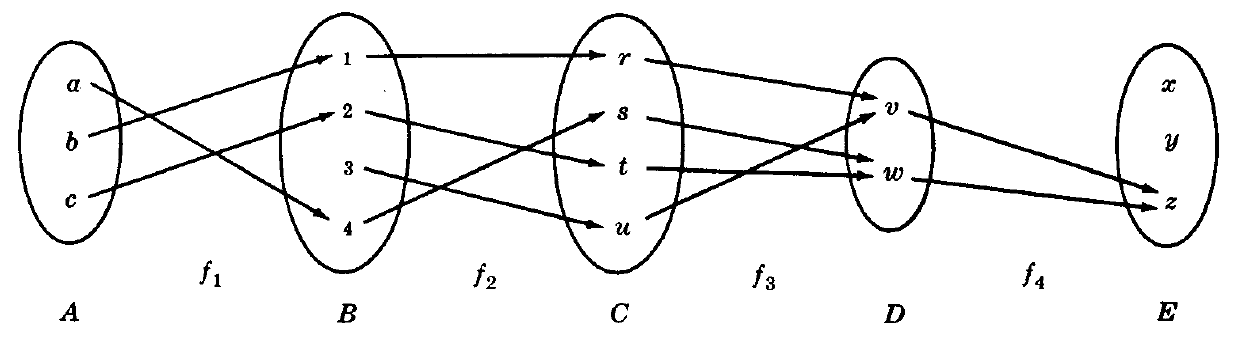
\includegraphics[width=10cm,keepaspectratio=true]{./md/MD02_IM01.png}
		% MD02_IM01.png: 0x0 pixel, 300dpi, 0.00x0.00 cm, bb=
		\label{fig:MD0201}
	\end{figure}
	
\end{problema}

\begin{figure}
	\centering
	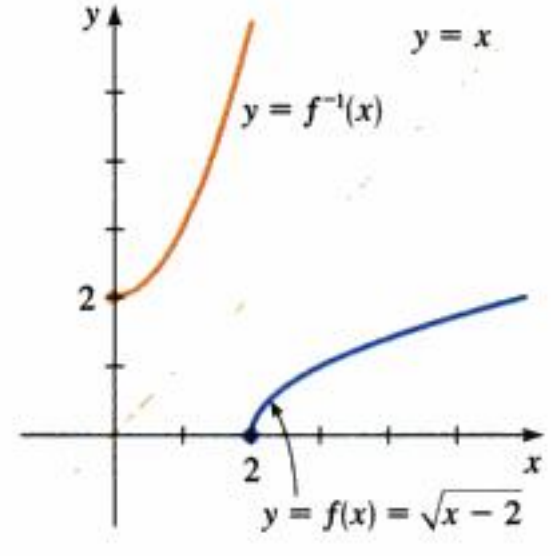
\includegraphics[height=8cm,keepaspectratio=true]{./md/MD02_sqrt_x-2.png}
	% MD02_sqrt_x-2.png: 0x0 pixel, 300dpi, 0.00x0.00 cm, bb=
	\label{fig:MD02_sqrt_x-2}
\end{figure}

\begin{figure}
	\centering
	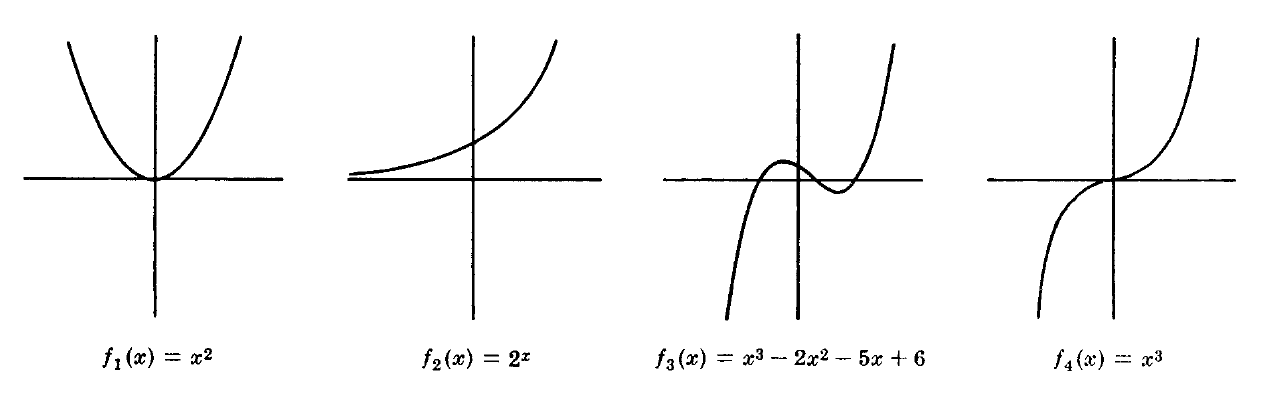
\includegraphics[width=10cm]{./md/MD02_IM02.png}
	% MD02_IM02.png: 0x0 pixel, 300dpi, 0.00x0.00 cm, bb=
	\label{fig:MD0202}
\end{figure}



\begin{problema}
	Encuentre la inversa de la función $f(x)=3x-2,$
\end{problema}




\begin{problema}
	Encuentre la inversa de $f(x)=\dfrac{x^{5}-3}{2}.$
\end{problema}




\begin{problema}
	Encuentre la inversa de $f(x)=\sqrt{x-2}.$
\end{problema}



\begin{problema}
	Considere las siguientes funciones $:\R \to \R$
	\begin{enumerate}
		\item $x \mapsto x^{2}$
		\item $x \mapsto 2^{x}$
		\item $x \mapsto x^{3}-2x^{2}-5x+6$
		\item $x \mapsto x^{3}$
	\end{enumerate}
	y determine si son $1:1,$ sobre o invertibles.
\end{problema}